% Options for packages loaded elsewhere
\PassOptionsToPackage{unicode}{hyperref}
\PassOptionsToPackage{hyphens}{url}
\PassOptionsToPackage{dvipsnames,svgnames,x11names}{xcolor}
%
\documentclass[
  a4paper,
  DIV=11,
  numbers=noendperiod]{scrartcl}

\usepackage{amsmath,amssymb}
\usepackage{iftex}
\ifPDFTeX
  \usepackage[T1]{fontenc}
  \usepackage[utf8]{inputenc}
  \usepackage{textcomp} % provide euro and other symbols
\else % if luatex or xetex
  \usepackage{unicode-math}
  \defaultfontfeatures{Scale=MatchLowercase}
  \defaultfontfeatures[\rmfamily]{Ligatures=TeX,Scale=1}
\fi
\usepackage{lmodern}
\ifPDFTeX\else  
    % xetex/luatex font selection
\fi
% Use upquote if available, for straight quotes in verbatim environments
\IfFileExists{upquote.sty}{\usepackage{upquote}}{}
\IfFileExists{microtype.sty}{% use microtype if available
  \usepackage[]{microtype}
  \UseMicrotypeSet[protrusion]{basicmath} % disable protrusion for tt fonts
}{}
\makeatletter
\@ifundefined{KOMAClassName}{% if non-KOMA class
  \IfFileExists{parskip.sty}{%
    \usepackage{parskip}
  }{% else
    \setlength{\parindent}{0pt}
    \setlength{\parskip}{6pt plus 2pt minus 1pt}}
}{% if KOMA class
  \KOMAoptions{parskip=half}}
\makeatother
\usepackage{xcolor}
\setlength{\emergencystretch}{3em} % prevent overfull lines
\setcounter{secnumdepth}{5}
% Make \paragraph and \subparagraph free-standing
\ifx\paragraph\undefined\else
  \let\oldparagraph\paragraph
  \renewcommand{\paragraph}[1]{\oldparagraph{#1}\mbox{}}
\fi
\ifx\subparagraph\undefined\else
  \let\oldsubparagraph\subparagraph
  \renewcommand{\subparagraph}[1]{\oldsubparagraph{#1}\mbox{}}
\fi


\providecommand{\tightlist}{%
  \setlength{\itemsep}{0pt}\setlength{\parskip}{0pt}}\usepackage{longtable,booktabs,array}
\usepackage{calc} % for calculating minipage widths
% Correct order of tables after \paragraph or \subparagraph
\usepackage{etoolbox}
\makeatletter
\patchcmd\longtable{\par}{\if@noskipsec\mbox{}\fi\par}{}{}
\makeatother
% Allow footnotes in longtable head/foot
\IfFileExists{footnotehyper.sty}{\usepackage{footnotehyper}}{\usepackage{footnote}}
\makesavenoteenv{longtable}
\usepackage{graphicx}
\makeatletter
\def\maxwidth{\ifdim\Gin@nat@width>\linewidth\linewidth\else\Gin@nat@width\fi}
\def\maxheight{\ifdim\Gin@nat@height>\textheight\textheight\else\Gin@nat@height\fi}
\makeatother
% Scale images if necessary, so that they will not overflow the page
% margins by default, and it is still possible to overwrite the defaults
% using explicit options in \includegraphics[width, height, ...]{}
\setkeys{Gin}{width=\maxwidth,height=\maxheight,keepaspectratio}
% Set default figure placement to htbp
\makeatletter
\def\fps@figure{htbp}
\makeatother

\KOMAoption{captions}{tableheading}
\makeatletter
\makeatother
\makeatletter
\makeatother
\makeatletter
\@ifpackageloaded{caption}{}{\usepackage{caption}}
\AtBeginDocument{%
\ifdefined\contentsname
  \renewcommand*\contentsname{Table of contents}
\else
  \newcommand\contentsname{Table of contents}
\fi
\ifdefined\listfigurename
  \renewcommand*\listfigurename{List of Figures}
\else
  \newcommand\listfigurename{List of Figures}
\fi
\ifdefined\listtablename
  \renewcommand*\listtablename{List of Tables}
\else
  \newcommand\listtablename{List of Tables}
\fi
\ifdefined\figurename
  \renewcommand*\figurename{Figure}
\else
  \newcommand\figurename{Figure}
\fi
\ifdefined\tablename
  \renewcommand*\tablename{Table}
\else
  \newcommand\tablename{Table}
\fi
}
\@ifpackageloaded{float}{}{\usepackage{float}}
\floatstyle{ruled}
\@ifundefined{c@chapter}{\newfloat{codelisting}{h}{lop}}{\newfloat{codelisting}{h}{lop}[chapter]}
\floatname{codelisting}{Listing}
\newcommand*\listoflistings{\listof{codelisting}{List of Listings}}
\makeatother
\makeatletter
\@ifpackageloaded{caption}{}{\usepackage{caption}}
\@ifpackageloaded{subcaption}{}{\usepackage{subcaption}}
\makeatother
\makeatletter
\@ifpackageloaded{tcolorbox}{}{\usepackage[skins,breakable]{tcolorbox}}
\makeatother
\makeatletter
\@ifundefined{shadecolor}{\definecolor{shadecolor}{rgb}{.97, .97, .97}}
\makeatother
\makeatletter
\makeatother
\makeatletter
\makeatother
\ifLuaTeX
  \usepackage{selnolig}  % disable illegal ligatures
\fi
\IfFileExists{bookmark.sty}{\usepackage{bookmark}}{\usepackage{hyperref}}
\IfFileExists{xurl.sty}{\usepackage{xurl}}{} % add URL line breaks if available
\urlstyle{same} % disable monospaced font for URLs
\hypersetup{
  pdftitle={BINF200 Assignment 2},
  pdfauthor={Multiple sequence analysis, phylogenetics, motif analysis},
  colorlinks=true,
  linkcolor={blue},
  filecolor={Maroon},
  citecolor={Blue},
  urlcolor={Blue},
  pdfcreator={LaTeX via pandoc}}

\title{BINF200 Assignment 2}
\author{Multiple sequence analysis, phylogenetics, motif analysis}
\date{2023-10-02}

\begin{document}
\maketitle
\ifdefined\Shaded\renewenvironment{Shaded}{\begin{tcolorbox}[sharp corners, breakable, borderline west={3pt}{0pt}{shadecolor}, interior hidden, boxrule=0pt, enhanced, frame hidden]}{\end{tcolorbox}}\fi

\hypertarget{deadline-grading-and-report}{%
\section{Deadline, grading and
report}\label{deadline-grading-and-report}}

The assignment is due \textbf{13 October 2023}.

The assignment is scored on \textbf{20 points} and counts towards
\textbf{10\% of the final grade}.

Your report should be a \textbf{single PDF file} that contains your
report text, code, and figures in a single document. The easiest
workflow is probably to run your analyses in a Jupyter or similar
notebook, and save the final notebook as a PDF file.

You \emph{may} work together, but you \emph{must} declare it in your
report.

Any use of ChatGPT or other generative AI tools \emph{must} be declared
in your report.

\hypertarget{background}{%
\section{Background}\label{background}}

In this compulsory assignment, you will perform bioinformatics analyses
covering multiple sequence alignment, phylogenetic tree construction and
motif finding. The assignment will cover practical use of
state-of-the-art tools, and also questions requiring programming. You
may use any programming language: Python, Julia, R, \ldots{}

\hypertarget{data}{%
\section{Data}\label{data}}

Download all files in the following OneDrive folder:

\url{https://universityofbergen-my.sharepoint.com/:f:/r/personal/tom_michoel_uib_no/Documents/public/BINF200/Coronavirus?csf=1\&web=1\&e=D5umem}

You should find the following files:

\begin{itemize}
\tightlist
\item
  \textbf{protein\_N\_data.fasta} - Sequences of the gene coding for
  coronavirus nucleocapsid (N) protein in a number of coronaviruses
\item
  \textbf{GCA\_011537005.1\_partial\_genomic.fasta} - Part of the
  BetaCoV/Wuhan/IPBCAMS-WH-02/2019 genome
\item
  \textbf{motifCountMatrix.csv} - Count matrix of a sequence motif
\end{itemize}

\hypertarget{tasks}{%
\section{Tasks}\label{tasks}}

\hypertarget{multiple-sequence-alignment-and-phylogenetic-tree-construction-for-the-coronavirus-nucleocapsid-protein-total-points-5}{%
\subsection{Multiple sequence alignment and phylogenetic tree
construction for the coronavirus nucleocapsid protein (Total points:
5)}\label{multiple-sequence-alignment-and-phylogenetic-tree-construction-for-the-coronavirus-nucleocapsid-protein-total-points-5}}

We will focus on different genera of corona viruses namely: alpha, beta,
gamma and delta. Their genomes, gene and protein sequences, together
with annotations and data reports are available from NCBI:

\begin{itemize}
\tightlist
\item
  Alpha coronavirus:
  \url{https://www.ncbi.nlm.nih.gov/datasets/taxonomy/693996/}
\item
  Beta coronavirus:
  \url{https://www.ncbi.nlm.nih.gov/datasets/taxonomy/694002/}
\item
  Gamma coronavirus:
  \url{https://www.ncbi.nlm.nih.gov/datasets/taxonomy/694013/}
\item
  Delta coronavirus:
  \url{https://www.ncbi.nlm.nih.gov/datasets/taxonomy/1159901/}
\end{itemize}

For simplicity, we will use data from only one important gene, that
encodes the coronavirus nucleocapsid (N) protein. This is a structural
protein that forms complexes with genomic RNA, interacts with the viral
membrane protein during virion assembly and plays a critical role in
enhancing the efficiency of virus transcription and assembly. You can
read more about it in the paper
\href{https://www.ncbi.nlm.nih.gov/pmc/articles/PMC8227405/}{\emph{The
SARS-CoV-2 Nucleocapsid Protein and Its Role in Viral Structure,
Biological Functions, and a Potential Target for Drug or Vaccine
Mitigation}}.

The datasets listed in Figure 1 were used to create
\textbf{protein\_N\_data.fasta}.

\begin{figure}

{\centering 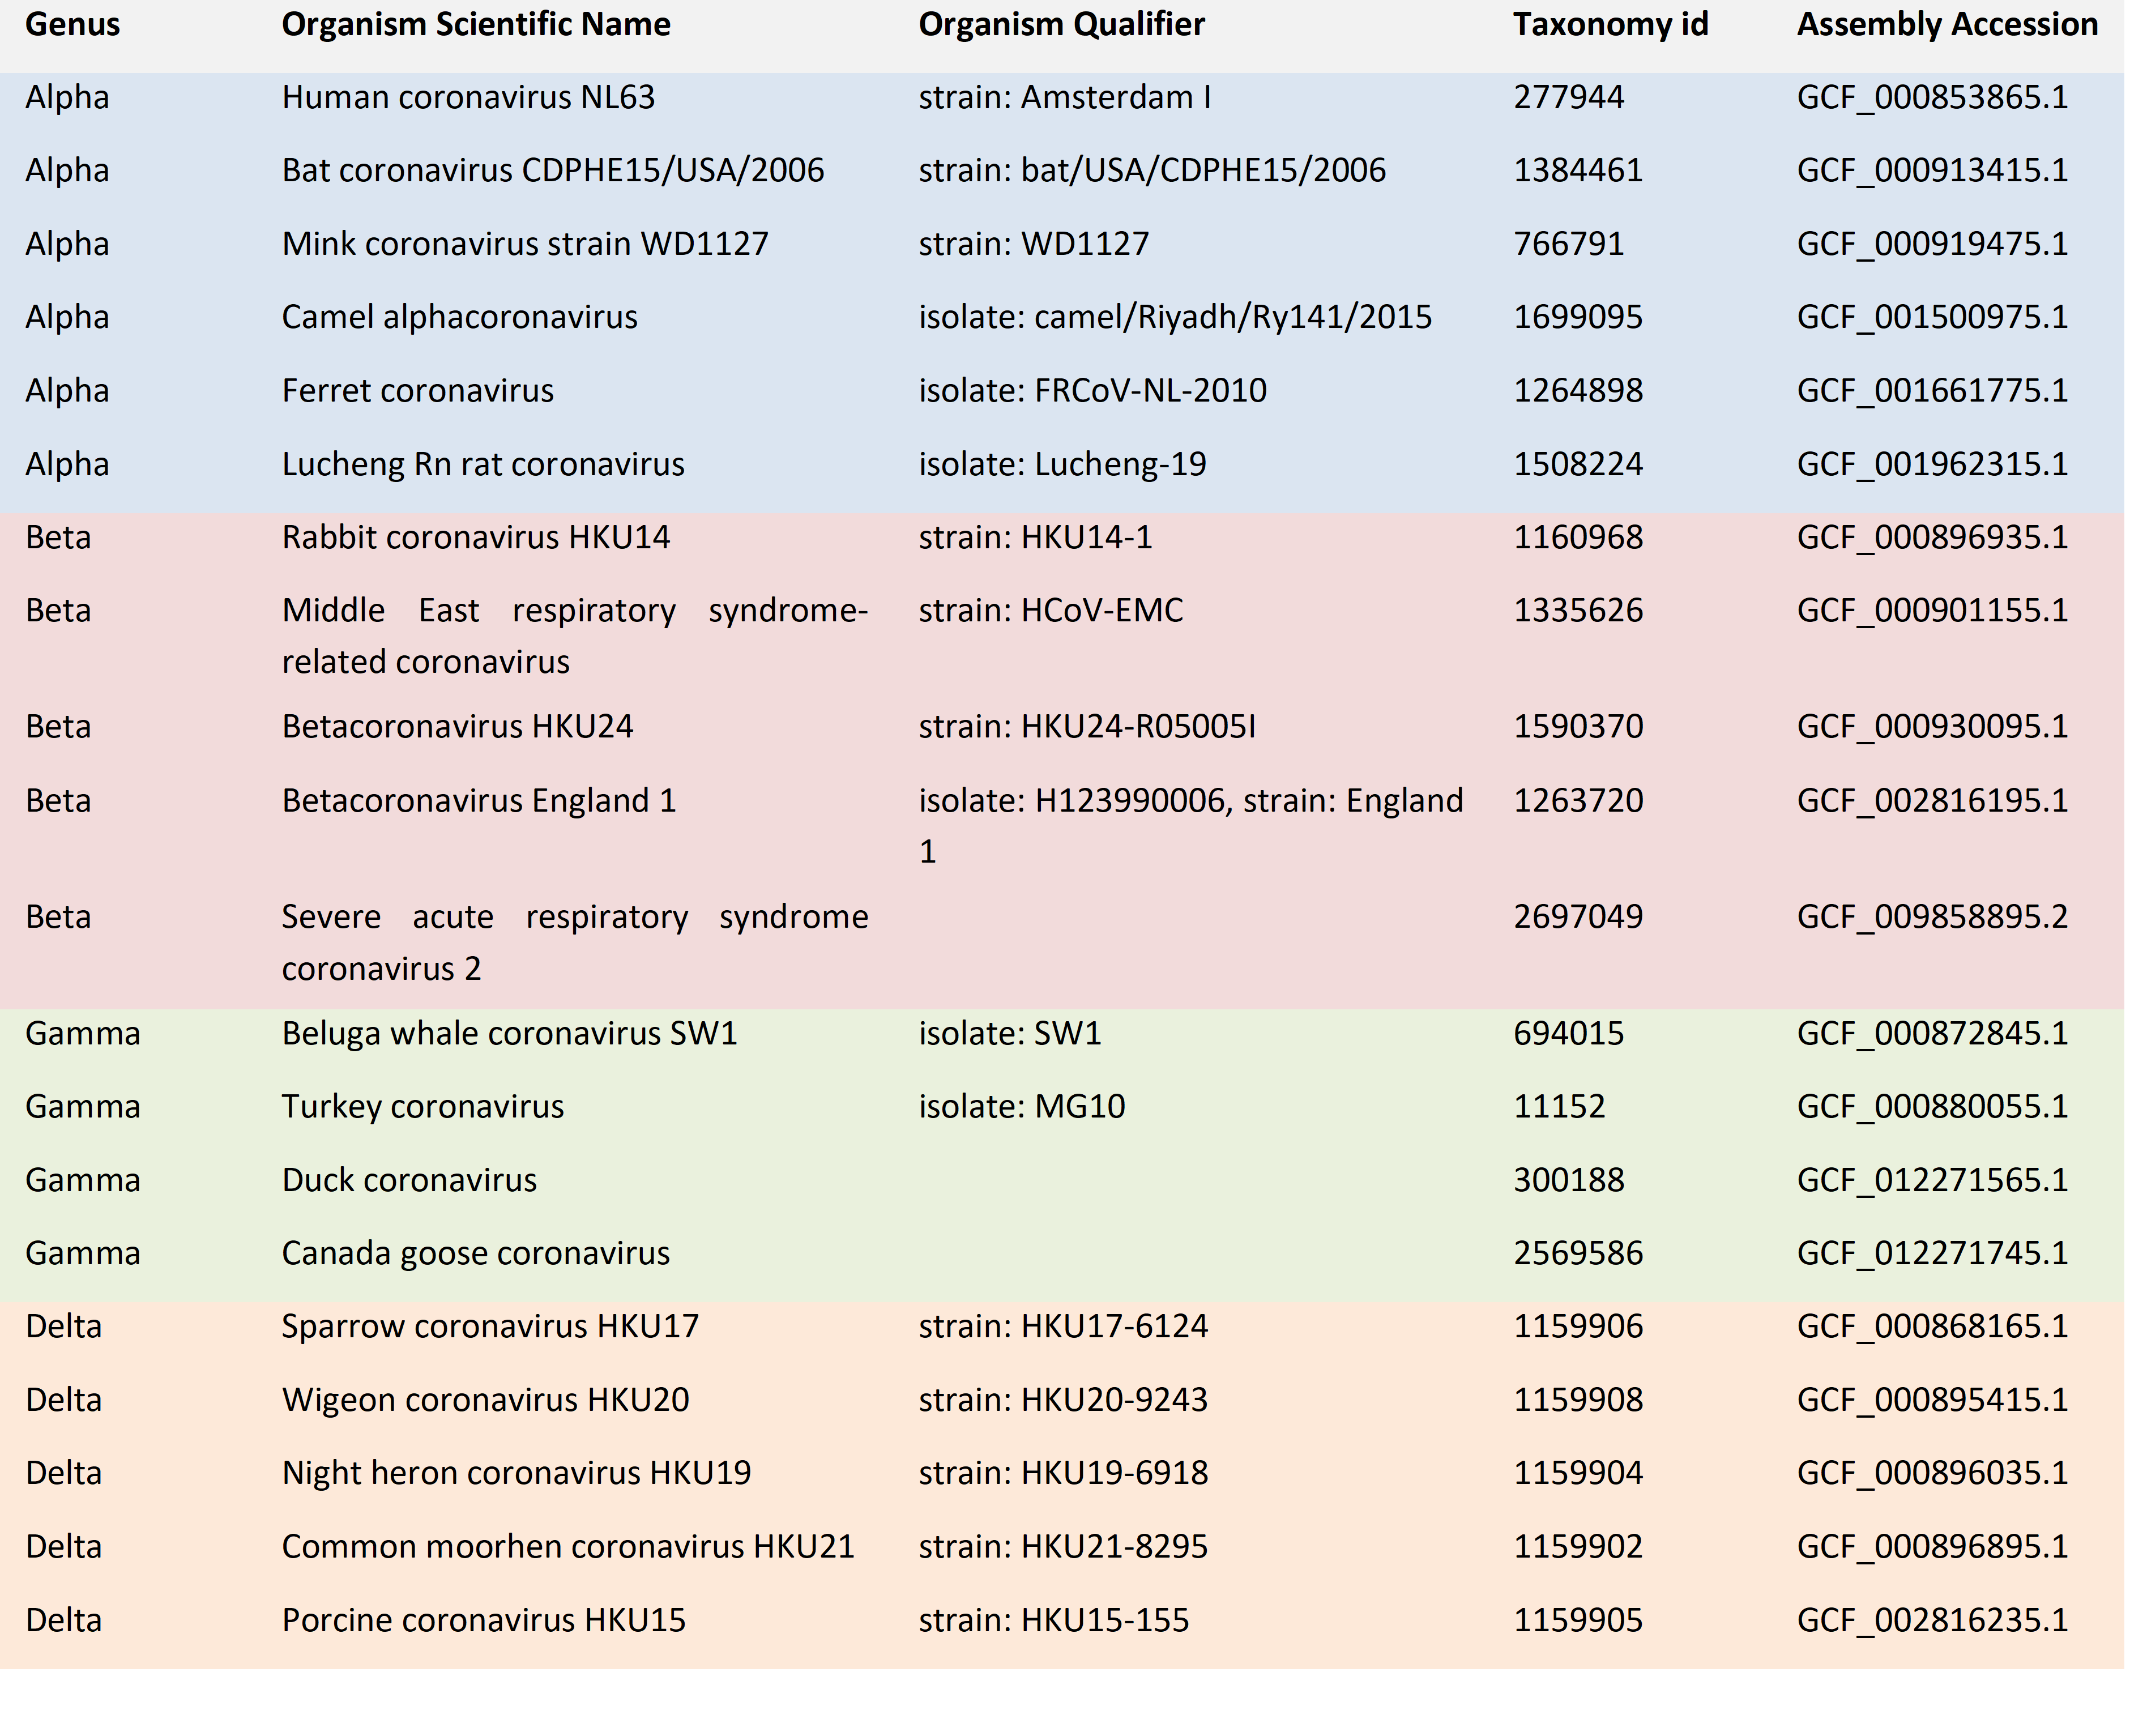
\includegraphics{assgn2_coronavirus_table.png}

}

\caption{Table of coronavirus source datasets}

\end{figure}

\hypertarget{parse-the-fasta-file-1-point}{%
\subsubsection{Parse the fasta file (1
point)}\label{parse-the-fasta-file-1-point}}

How many sequences are contained in the file
\textbf{protein\_N\_data.fasta}?

List the names of the sequences.

\hypertarget{find-protein-n-in-a-specific-coronavirus-genome-1-point}{%
\subsubsection{Find protein N in a specific coronavirus genome (1
point)}\label{find-protein-n-in-a-specific-coronavirus-genome-1-point}}

From the sequences in \textbf{protein\_N\_data.fasta}, find the sequence
for which the first letter in its name is closest in the alphabet to the
\textbf{first letter in your first name}. If there are multiple
sequences starting with the same letter, pick one arbitrarily. For the
selected sequence:

\begin{itemize}
\tightlist
\item
  Find the assembly accession ID in the table above.
\item
  Go to the NCBI website (cf.~links above) and find the corresponding
  genome assembly.
\item
  What are the genomic coordinates (start and end position) of gene N in
  this genome? (Hint: follow the RefSeq link)
\end{itemize}

\hypertarget{multiple-sequence-alignment-1-point}{%
\subsubsection{Multiple sequence alignment (1
point)}\label{multiple-sequence-alignment-1-point}}

Build a multiple sequence alignment for the \textbf{protein\_N\_data}
using a multiple sequence alignment tool of your choice. (Hint: check
out the services provided by EMBL's European Bioinformatics Institute
(EMBL-EBI).)

\hypertarget{sec-phylo-1}{%
\subsubsection{Phylogenetic tree reconstruction (1
point)}\label{sec-phylo-1}}

Based on the results from the previous step, build a phylogenetic tree.
(Hint: at this stage it is not required to make an ``advanced tree'',
providing a simple tree is enough). Save the image of the
phylogenetic/guide tree.

\hypertarget{interpretation-1-point}{%
\subsubsection{Interpretation (1 point)}\label{interpretation-1-point}}

Based on the results from the previous two steps, what do you see?
Elaborate with a small text (3-4 lines): Explain what you observe from
the multiple sequence alignment itself (hint: check the number of
conserved sites), and give a short interpretation of the phylogenetic
tree you have constructed.

\hypertarget{step-by-step-multiple-sequence-alignment-and-phylogenetic-tree-construction-using-upgma-total-points-10}{%
\subsection{Step-by-step multiple sequence alignment and phylogenetic
tree construction using UPGMA (Total points:
10)}\label{step-by-step-multiple-sequence-alignment-and-phylogenetic-tree-construction-using-upgma-total-points-10}}

\hypertarget{compute-pairwise-similarities-2-points}{%
\subsubsection{Compute pairwise similarities (2
points)}\label{compute-pairwise-similarities-2-points}}

Use the Needleman-Wunsch (dynamic programming) pairwise alignment
algorithm to build a matrix of global alignment scores for each pair of
sequences in \textbf{protein\_N\_data.fasta}. You can choose between
multiple options:

\begin{itemize}
\tightlist
\item
  Implement the Needleman-Wunsch algorithm yourself. (Hint: You have
  probably done this already in BINF100)
\item
  Use an existing implementation of the algorithm. (Hint: Check
  biopython, biojulia)
\item
  Use the \emph{needleall} command line program from the EMBOSS suite.
  (Hint: You installed the whole EMBOSS suite for Assignment 1.)
\item
  Use a webserver such as EMBL-EBI's EMBOSS Needle service. (Hint:
  Manually inputting every pair of sequences will be extremely tedious,
  though they do provide APIs.)
\end{itemize}

\hypertarget{generate-a-pairwise-distance-matrix-4-points}{%
\subsubsection{Generate a pairwise distance matrix (4
points)}\label{generate-a-pairwise-distance-matrix-4-points}}

Generate a distance matrix from the score matrix you have created in the
previous step. For this task we will use Feng \& Doolittle's
formulation, and we will compute the distance \(D\) using formula:

\[
D = -\log S_{eff} = -\log \frac{S_{obs}-S_{rand}}{S_{max} - S_{rand}}
\]

where

\begin{itemize}
\tightlist
\item
  \(S_{obs}\) is the observed pairwise alignment score
\item
  \(S_{max}\) is the best alignment score for both sequences, obtained
  by taking the average of the score of aligning either sequence to
  itself
\item
  \(S_{rand}\) is the expected (average) score for aligning two random
  sequences of the same length and residue composition, obtained by
  random shuffling the nucleotide composition of the two sequences.
  (Hint: more info about the Feng \& Doolittle can be found at this URL:
  \url{https://rna.informatik.uni-freiburg.de/Teaching/index.jsp?toolName=Feng-Doolittle})
\end{itemize}

Compute \(S_{rand}\) by taking the average score of \textbf{10} pairwise
alignments between random sequences with the same sequence compositions
as the original sequences.

\hypertarget{generate-a-guide-tree-of-phylogenetic-relationships-2-points}{%
\subsubsection{Generate a ``guide tree'' of phylogenetic relationships
(2
points)}\label{generate-a-guide-tree-of-phylogenetic-relationships-2-points}}

Generate a ``guide tree'' of phylogenetic relationships from the
pairwise distance matrix you have created in the previous step using the
UPGMA method. You can choose between multiple options:

\begin{itemize}
\tightlist
\item
  Implement the UPGMA hierarchical clustering algorithm yourself. (Hint:
  You can represent the tree as a binary tree, either implementing a
  tree class yourself, or using an existing data structure.)
\item
  Use an existing implementation of the algorithm. (Hint: UPGMA is more
  commonly known as hierarchical clustering with average linkage. Check
  SciPy or similar packages for other languages.)
\end{itemize}

\hypertarget{interpret-your-results-2-points}{%
\subsubsection{Interpret your results (2
points)}\label{interpret-your-results-2-points}}

Visualize your guide tree and compare it to the phylogenetic tree
constructed in Section~\ref{sec-phylo-1}. Elaborate with a small text
(3-4 lines) to explain what you observe.

\hypertarget{sequence-motifs-total-points-5}{%
\subsection{Sequence motifs (Total points:
5)}\label{sequence-motifs-total-points-5}}

Do simple motif searching on corona virus sequences using the input
dataset (\textbf{protein\_N\_data.fasta}) we have already analysed.

\hypertarget{meme-analysis-1-point}{%
\subsubsection{MEME analysis (1 point)}\label{meme-analysis-1-point}}

Connect to the MEME platform at \url{https://meme-suite.org/}.

\begin{itemize}
\tightlist
\item
  Find the MEME motif discovery tool.
\item
  Input \textbf{protein\_N\_data.fasta} to discover enriched motifs in
  this set of sequences, allowing for zero or one motif occurrence per
  sequence and finding upto 5 motifs. Which discovery mode, sequence
  alphabet, and site distribution options do you select?
\end{itemize}

Open and download the \textbf{MEME HTML output file} and include the
sequence logos of the motifs found in your report.

\hypertarget{convert-count-matrix-to-pwm-2-points}{%
\subsubsection{Convert count matrix to PWM (2
points)}\label{convert-count-matrix-to-pwm-2-points}}

We will work with a 20-nucleotide subset of the first motif found by the
MEME software, given by the count matrix:

\begin{figure}

{\centering 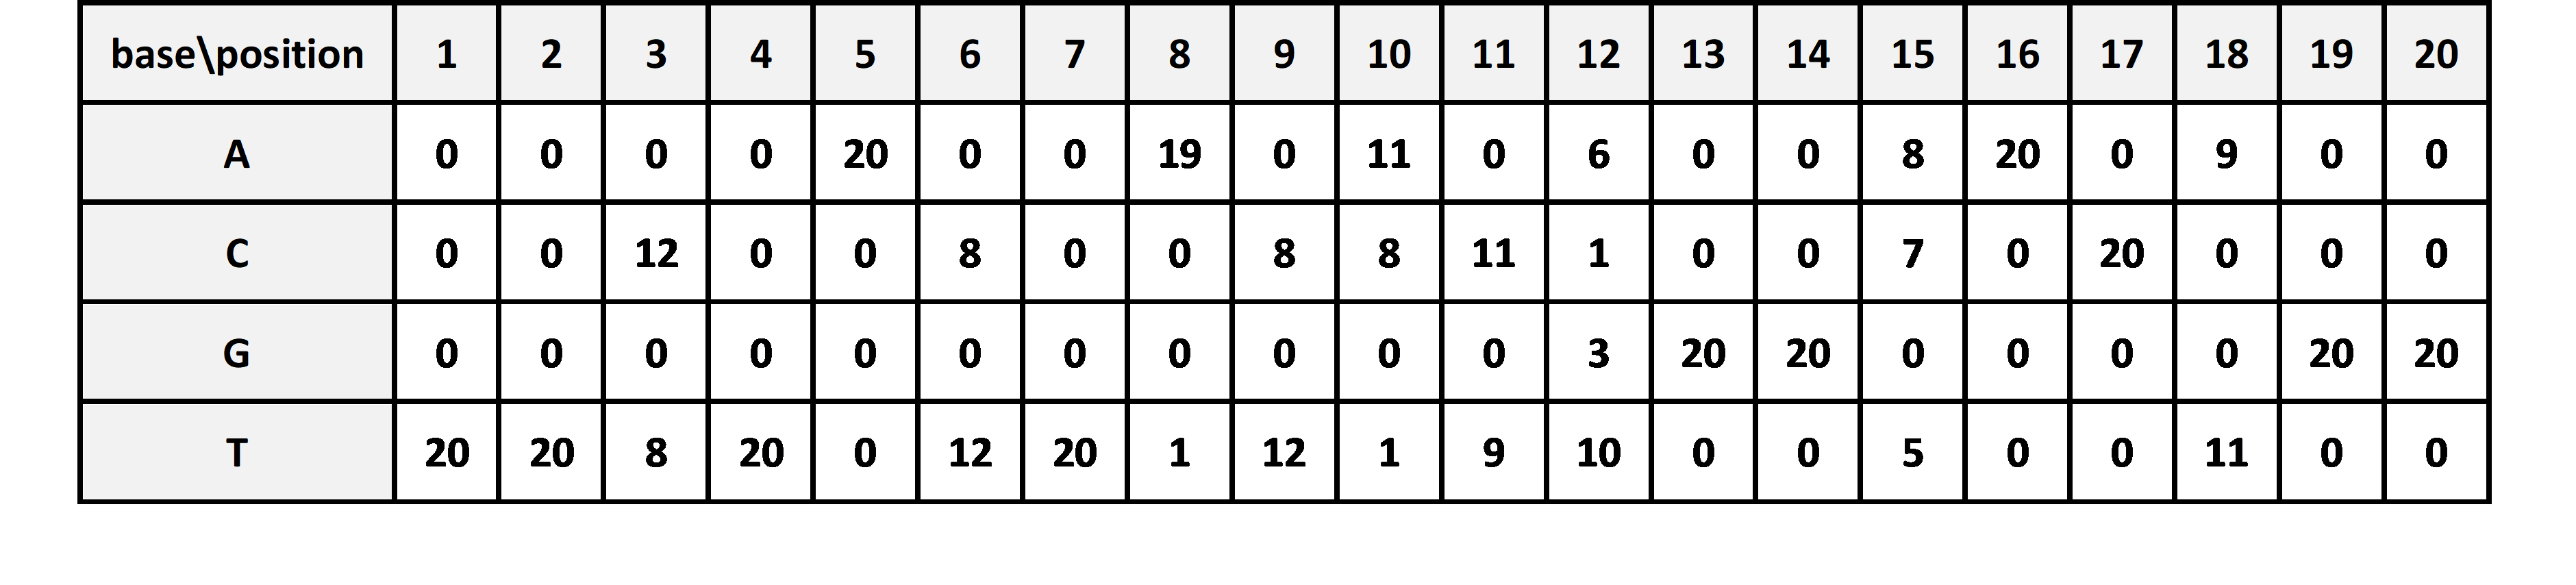
\includegraphics{assgn2_motif_counts.png}

}

\caption{Motif count matrix}

\end{figure}

The count matrix is also available as a file
\textbf{motifCountMatrix.csv}.

\begin{enumerate}
\def\labelenumi{\arabic{enumi}.}
\item
  Compare the count matrix against your sequence logos and mark the
  20-nucleotide window corresponding to this count matrix in the right
  logo.
\item
  Convert the count matrix to a position-specific probability matrix
  (PPM) \(P\). To avoid zeros in the PPM, we add \emph{pseudo-counts}
  and define

  \[
  P_{k,i} = \frac{\text{Count}_{k,i} + 0.25 * \sqrt{N}}{N + \sqrt{N}},
  \]

  where \(\text{Count}_{k,i}\) is the value of the count matrix for
  nucleotide \(k\) in motif position \(i\), and \(N\) is the number of
  sequences in \textbf{protein\_N\_data.fasta} (Hint: Count the totals
  in each column of the count matrix).
\item
  Convert the PPM matrix to a position-specific weight matrix (PWM)
  \(W\) using the formula

  \[
  W_{k,i} = \log_2 \frac{P_{k,i}}{0.25}
  \]

  What would be the value of \(W\) for a random background site with
  equal counts for all nucleotides and using the pseudo-count formula
  above to compute the random probabilities?
\end{enumerate}

\hypertarget{scan-a-coronavirus-genome-for-motif-occurrences-2-points}{%
\subsubsection{Scan a coronavirus genome for motif occurrences (2
points)}\label{scan-a-coronavirus-genome-for-motif-occurrences-2-points}}

Scan part of the BetaCoV/Wuhan/IPBCAMS-WH-02/2019 genome (the sequence
in the file \textbf{GCA\_011537005.1\_partial\_genomic.fasta}) and score
all possible motif occurrences. Use the sliding window approach
presented in the lecture and report (figure) both the log-odds score and
the odds of each possible motif starting position in the genome
sequence.

Elaborate with a small text (3-4 lines) to explain what you observe.



\end{document}
